% !TeX TXS-program:compile = txs:///pdflatex/[--shell-escape]

\documentclass[12pt,a4paper]{scrartcl}
\usepackage[utf8]{inputenc}
\usepackage[english,russian]{babel}
\usepackage{indentfirst}
\usepackage{misccorr}
\usepackage{graphicx}
\usepackage{amsmath}
\usepackage{hyperref}
\usepackage{float}
\usepackage{minted} %для вставки кода в документ

\begin{document}

\section{Использование GPU для различных криптографических приложений}

Достаточно часто, решая прикладные криптографические задачи, приходится перебирать некоторое конечное количество значений на одинаковой схеме (подбор пароля по его хэшу, подбор пароля по развертке ключа и по проведению процедуры расшифровывания симметричного алгоритма и т.д.).

Задачи такого плана очень хорошо ложатся на архитектуру SIMD. 
Кратко опишем основные архитектуры, которые понадобятся нам далее:

SISD - (Single Instruction Single Data) - архитектура, при которой один поток инструкций выполняется над одним потоком данных. Данная архитектура больше всего распространена, так как она является архитектурой одноядерного процессора CPU.

SIMD - (Single Instruction Multiple Data) - архитектура, при которой один поток инструкций выполняется над несколькими потоками данных. То есть код выполняемой программы одинаковый для всех потоков данных, а сами значения в этих данных различны. Типичным представителем данной архитектуры является GPU (Graphics Processing Unit).

Почему же именно SIMD так хорош для проведения подбора паролей? Потому что большинство криптографических алгоритмов являются не сильно ветвистыми (то есть в них нет большой вариативности действий в зависимости от входных данных), и поэтому в один момент времени будут выполняться одинаковые шаги алгоритма для разных потоков, если их запустить параллельно. 

\subsection{Сравнение CPU и GPU}


Первый вопрос, который должен задать каждый перед применением GPU для решения своих задач — а для каких целей хорош GPU, когда стоит его применять? Для ответа нужно определить 2 понятия:

\begin{itemize}
	\item \textit{Задержка} (latency) — время, затрачиваемое на выполнение одной инструкции/операции.
	\item \textit{Пропускная способность} — количество инструкций/операций, выполняемых за единицу времени.
\end{itemize}

Для того, чтобы разобраться в этих терминах, приведем простой пример: допустим, мы имеем легковой автомобиль со скоростью 90 км/ч и вместимостью 4 человека, и автобус со скоростью 60 км/ч и вместимостью 20 человек. Если за операцию принять перемещение 1 человека на 1 километр, то задержка легкового автомобиля — 3600/90=40с — за столько секунд 1 человек преодолеет расстояние в 1 километр, пропускная способность автомобиля — 4/40=0.1 операций/секунду; задержка автобуса — 3600/60=60с, пропускная способность автобуса — 20/60=0.3(3) операций/секунду.

Так вот, CPU в данной ситуации можно сравнить с автомобием, а GPU — с автобусом: он имеет большую задержку но также и большую пропускную способность. Если для вашей задачи задержка каждой конкретной операции не настолько важна как количество этих операций в секунду — стоит рассмотреть применение GPU.

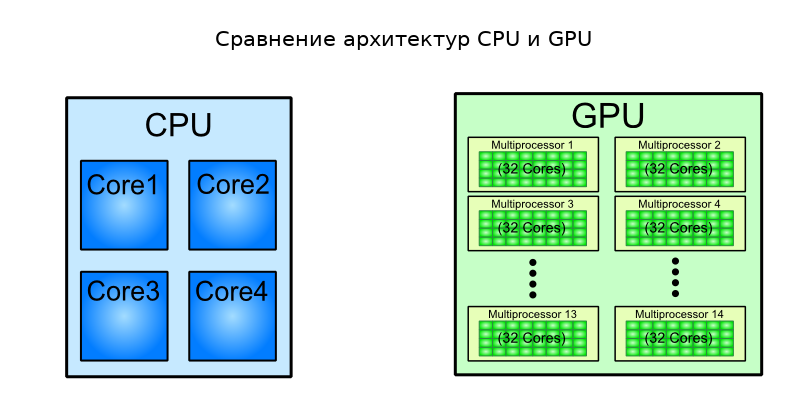
\includegraphics[scale=0.5]{./pictures/Arch.png}

Наши однотипные вычисления при их массовости отлично выписываются в класс таких задач - попробуем организовать их расчет на GPU. 

\subsection{Базовые понятия и термины CUDA}

Итак, разберемся с терминологией CUDA:

\begin{itemize}
\item Устройство (device) — GPU. Выполняет роль «подчиненного» — делает только то, что ему говорит CPU.
\item Хост (host) — CPU. Выполняет управляющую роль — запускает задачи на устройстве, выделяет память на устройстве, перемещает память на/с устройства. И да, использование CUDA предполагает, что как устройство так и хост имеют свою отдельную память.
\item Ядро (kernel) — задача, запускаемая хостом на устройстве.
\end{itemize}


При использовании CUDA вы просто пишете код на языке программирования С или С++, после чего компилятор CUDA сгенерирует код отдельно для хоста и отдельно для устройства.

Небольшая оговорка: код для устройства должен быть написан только на языке C с некоторыми 'CUDA-расширениями'.

\subsubsection{Основные этапы CUDA-программы}

Рассмотрим общую схему работы любой программы, написанной для CUDA:

\begin{enumerate}
	\item Хост выделяет нужное количество памяти на устройстве.
	\item Хост копирует данные из своей памяти в память устройства.
	\item Хост стартует выполнение определенных ядер на устройстве.
	\item Устройство выполняет ядра.
	\item Хост копирует результаты из памяти устройства в свою память.
\end{enumerate}

Естественно, для наибольшей эффективности использования GPU нужно чтобы соотношение времени, потраченного на работу ядер, к времени, потраченному на выделение памяти и перемещение данных, было как можно больше, а также желательно, чтобы из памяти видеокарты в память хоста и наоборот за один раз копировалось как можно больше информации - это повысит скорость копирования.

\subsubsection{Ядра}

Рассмотрим более детально процесс написания кода для ядер и их запуска. Важный принцип — ядра пишутся как (практически) обычные последовательные программы — то-есть вы не увидите создания и запуска потоков в коде самих ядер. Вместо этого, для организации параллельных вычислений GPU запустит большое количество копий одного и того же ядра в разных потоках — а точнее, вы сами говорите сколько потоков запустить. И да, возвращаясь к вопросу эффективности использования GPU — чем больше потоков вы запускаете (при условии что все они будут выполнять полезную работу) — тем лучше.
Код для ядер отличается от обычного последовательного кода в таких моментах:

Внутри ядер вы имеете возможность узнать «идентификатор» или, проще говоря, позицию потока, который сейчас выполняется — используя эту позицию мы добиваемся того, что одно и то же ядро будет работать с разными данными в зависимости от потока, в котором оно запущено. 
В некоторых случаях в коде ядра необходимо использовать различные способы синхронизации, но конкретно наша задача не будет требовать таких ухищрений.


Каким же образом мы задаем количество потоков, в которых будет запущено ядро? Поскольку GPU это все таки Graphics Processing Unit, то это, естественно, повлияло на модель CUDA, а именно на способ задания количества потоков:

Сначала задаются размеры так называемой сетки (grid) в 3D координатах: grid\_x, grid\_y, grid\_z. В результате, сетка будет состоять из grid\_x*grid\_y*grid\_z блоков.
Потом задаются размеры блока в 3D координатах: block\_x, block\_y, bloc\_z. В результате, блок будет состоять из block\_x*block\_y*block\_z потоков. Итого, имеем grid\_x*grid\_y*grid\_z*block\_x*block\_y*block\_z потоков. Важное замечание — максимальное количество потоков в одном блоке ограничено и зависит от модели GPU — типичны значения 512 (более старые модели) и 1024 (более новые модели, как на машине автора статьи).
Внутри ядра доступны переменные threadIdx и blockIdx с полями x, y, z — они содержат 3D координаты потока в блоке и блока в сетке соответственно. Также доступны переменные blockDim и gridDim с теми же полями — размеры блока и сетки соответственно.


\textbf{Источник информации:}

\href{https://habr.com/ru/company/epam_systems/blog/245503/}{https://habr.com/ru/company/epam\_systems/blog/245503/}



\subsection{Установка CUDA development toolkit на ОС ubuntu 20.04}

Для работы с видеокартой нам нужно получить к ней прямой доступ, поэтому нам нужно иметь ОС с доступом к ней; при этом нужно учитывать, что это железо очень капризное и очень специфичное в работе. 

В общем случае можно работать с CUDA и в Windows, но так как мне привычнее работать в линукс-образных системах, то я установил ubuntu 20.04 второй системой (обойтись виртуальной машиной не получится, так как из решений под Windows нам подойдет только Hyper-V (которая не входит в обычную версию ОС), потому что только она умеет прокидывать видеокарту напрямую в ВМ, а для qemu в Windows не хватает некоторых драйверов, как выяснилось опытным путем. Vmware и Virtualbox тоже не умеют прокидывать видеокарту напрямую). Поэтому ниже я последовательно опишу действия, которые позволили мне правильно установить CUDA development toolkit.

Для начала я установил  ОС  ubuntu 20.04, не обновляя её при установке, после чего перешел с ядра 5.8 на более стабильное ядро 5.4 следующими командами:

\begin{enumerate}
	\item \textit{sudo apt install --install-recommends linux-generic} - скачивание некоторых зависимостей и заголовков для ядра 5.4
	\item \textit{sudo update-grub} - обновление grub, чтобы в меню загрузки можно было выбирать нужное ядро в расширенных настройках запуска ubuntu
	\item \textit{sudo reboot now} - перезапуск системы из консоли
	\item \textit{uname -r} - вывод в консоль версии ядра
\end{enumerate}


Далее рассмотрим последовательность действий для установки самого тулкита CUDA:

\begin{enumerate}
	\item \textit{sudo apt install gcc python3-dev python3-pip libxml2-dev libxslt1-dev zlib1g-dev g++} - установка некоторых компонентов, которые могут пригодится нам
	\item \textit{sudo apt-get install nvidia-cuda-toolkit} - усановка самого тулкита из репозиториев ubuntu (самый лаконичный способ установки, на мой взгляд).
	\item \textit{sudo add-apt-repository ppa:graphics-drivers/ppa} - добавление репозиториев драйверов в базу репозиториев инсталятора
	\item \textit{sudo ubuntu-drivers devices} - данная команда покажет нам рекомендуемую версию драйверов для нашей видеокарты - у меня это версия 460
	\item \textit{sudo apt install nvidia-driver-460} - установка самих драйверов для видеокарты
	\item \textit{sudo apt install nvidia-utils-460} - установка некоторого дополнительного окружения для драйверов нашей видеокарты
	\item \textit{nvidia-smi} - проверка драйверов (установились ли они)
\end{enumerate}

Информация о данной последовательности действий была собрана из большого количества различных мануалов и собственного опыта, поэтому первоисточники привести достаточно проблематично.

\subsection{Логика работы моей лаборатории}

Я написал лабораторный стенд, который позволяет количественно оценить возможности вашей машины при использовании CPU и GPU на максимум по перебору хэшей SHA1 для всех возможных 6-ти буквенных ключей (используется только английский строчный алфавит без цифер), что составляет около 300 млн различных паролей. 

Приятной особенностью данного стенда является тот факт, что на GPU и на CPU запускается одинаковая реализация SHA1, то есть мы проверяем одинаковый код на разных архитектурах процессора, что делает результаты эксперимента более интересными.


\subsection{Логика работы компонентов лаборатории}

Пароли генерируются с помощью python-скрипта следующим образом: 

В каждый созданный файл в папочку \textit{./keys/} кладется количество ключей, которое не может превышать указанного в скрипте значения. Для примера я решил генерировать все возможные комбинации английского строчного алфавита длины 6.

После запуска bash-скрипта \textit{./run.sh} из корневого каталога (который генерирует ключи), мы можем переместиться в каталог CPU или GPU, чтобы соответсвоенно запустить процесс восстановления парольной фразы по известному хэшу (запуская скрипт \textit{./CPU/run.sh} или \textit{./GPU/run.sh} соответственно) с помощью CPU или GPU.\\

Рассмотрим работу программы восстановления пароля на GPU:

Основными её компонентами являются скрипты \textit{./GPU/main.cu} и  \textit{./GPU/info\_about\_GPU.cu}, а также подпапка \textit{./sha1/}, в которой хранятся скрипты, отвечающие за расчет хэш-функции SHA1.

В файле \textit{./GPU/info\_about\_GPU.cu} содержится функция, которая выводит информацию об имеющейся в ПК видеокарте и выдает на выходе значение, которое равно количеству нитей в сетке (в моём случае это число равно 1024).

Листинг программы \textit{./GPU/main.cu} будет приведен ниже.

Кратко опишем логику его работы:
он принимает на вход хэш в верхнем регистре (или любое другое значение, которое мы хотим получить, выполняя над данными нам ключами преобразование, которое мы запрограммировали - в нашем случае это хэш - функция SHA1). Далее программа сама открывает по очереди все файлы из папки \textit{./keys/}, ммапит их в оперативную память (для более быстрого доступа) и отдает их видеокарте, которая в свою очередь рассчитывает хэш для каждого ключа и сравнивает с переданным через командную строку значением. Если найдется нужный хэш, то видеокарта ставит в соответствующую ячейку выходного массива '1', если совпадения не произошло - то '0'. Если произошла ошибка, то элемент массива примет значение '2'. 

Программа автоматически определяет количество файлов с ключами и количество ключей в каждом из них, а также размер этих ключей - поэтому все ключи в одном файле всегда должны иметь одинаковую длину и заканчиваться символом перевода строки.

Данную лабораторию можно использовать и для паролей разной длины - но при этом пароли с разными длинами кладутся в разные файлы. Так что можно генерировать пароли, подчиняясь этому правилу и правилу о том, что после каждого пароля должен стоять $'\backslash n'$.


Теперь обратимся к файлу \textit{./GPU/sha1/sha1.cu}.

В нем находится код программы, который работает в каждом ядре видеокарты и рассчитывает хэш для определенного ключа, который вычисляется по смещению z. Для вычисления хэша я использовал реализацию из интернета, ссылку на которую я оставлю в листинге программы.

Содержимое программы из папки \textit{./CPU/} почти полностью повторяет ранее описанные программы, только из них убраны модификаторы функций и добавлена \textit{\#pragma} и библиотека для работы с OpenMP (также в bash-скрипте изменен компилятор и добавлен необходимый флаг).

\subsection{Результаты работы}

Тестирование программ дало нам следующие результаты:

Время выполнения расчетов на GPU:

\begin{center}
	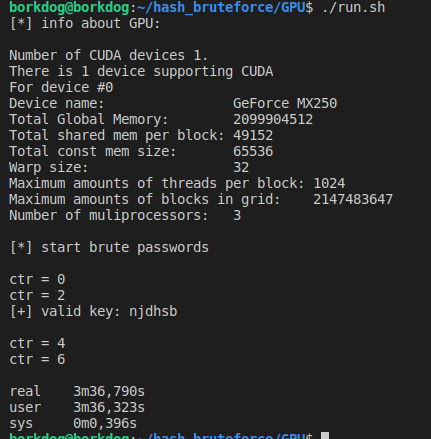
\includegraphics[scale=0.5]{./pictures/GPU.png}
\end{center}

Время, затраченное для расчетов на CPU в однопоточном режиме:

\begin{center}
	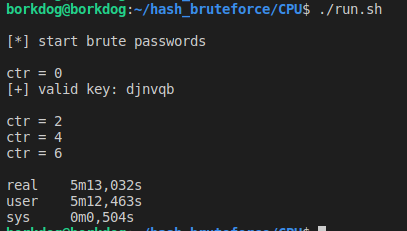
\includegraphics[scale=0.6]{./pictures/CPU_without_openMP.png}
\end{center}

Время, затраченное для расчетов на CPU с распараллеливанием на OpenMP:

\begin{center}
	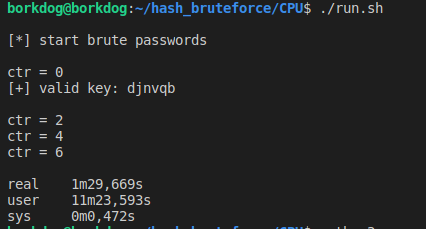
\includegraphics[scale=0.6]{./pictures/CPU.png}
\end{center}

Как мы и предполагали, видеокарта работает быстрее процессора, когда мы не используем многопоточность; но как только мы начинаем использовать её, то чувствуется заметная разница в скорости выполнения вычислений - скорее всего код, который я написал, не так сильно оптимизирован под GPU, как требуется. Также это может быть связано с тем, что видеокарта в моём ноутбуке просто изначально слабее, чем 8-ми ядерный процессор intel core i7, поэтому мы можем наблюдать превосходство по скорости  CPU над GPU.

\subsection{Плюсы использования GPU совместно с CPU, основываясь на результатах проведенной работы}

Используя результаты работы программ, можно выделить следующие плюсы работы с GPU:

Можно использовать много устройств GPU в одном компьютере под управлением одного CPU, что повысит производительность вычислений на стандартном ПК (подсоединять дополнительные процессоры CPU сложнее, чем устройства GPU).

Также можно комбинировать перебор на CPU и GPU, чтобы использовать мощности железа на максимум
(в таком режиме работы желательно использовать дополнительное охлаждение ноутбука или ПК, при этом (если это ноутбук) - использовать питание от сети, чтобы не расходовать ресурс батарейки).

\subsection{Листинги программ}



\underline{Скрипт ./GPU/main.cu:}

\inputminted[tabsize=4,obeytabs,fontsize=\footnotesize]{cuda}{../GPU/main.cu}

\underline{Скрипт ./GPU/info\_about\_GPU.cu:}

\inputminted[tabsize=4,obeytabs,fontsize=\footnotesize]{cuda}{../GPU/info_about_GPU.cu}

\underline{Скрипт ./GPU/sha1/sha1.cu:}

\inputminted[tabsize=4,obeytabs,fontsize=\footnotesize]{cuda}{../GPU/sha1/sha1.cu}

\underline{Скрипт ./run.sh:}

\inputminted[tabsize=4,obeytabs,fontsize=\footnotesize]{bash}{../run.sh}

\underline{Скрипт ./GPU/run.sh:}

\inputminted[tabsize=4,obeytabs,fontsize=\footnotesize]{bash}{../GPU/run.sh}

\underline{Скрипт ./CPU/run.sh:}

\inputminted[tabsize=4,obeytabs,fontsize=\footnotesize]{bash}{../CPU/run.sh}

Полный набор исходных кодов программ для лаборатории можно найти на моём github:

\href{https://github.com/Respman/CUDA_for_crypto}{https://github.com/Respman/CUDA\_for\_crypto}


\end{document}